\documentclass{article}
\usepackage{enumitem}
\usepackage{amsmath}
\usepackage{multirow}
\usepackage{graphicx}
\usepackage{subcaption}
\usepackage{float}

\title{CSE200: Online-1 on \LaTeX}
\author{Arunavo Anirban Aikko}
\date{January 11, 2026}

\begin{document}
\maketitle

\section{Introduction}
High-quality technical writing relies on \textbf{accuracy} and \emph{organized presentation} to convey complex concepts clearly. In this example, we show how to combine \textbf{text}, \textit{tables}, \underline{formulas} and {\large graphics} to create a coherent document.

Employing \textbf{distinct section titles}, \textit{well-structured lists} and \underline{key phrases} helps the reader follow the content effortlessly. Furthermore, careful use of {\small font variations}, inline expressions $(y_i, z_j)$ and deliberate spacing enhances the professional apperance of the document.

\section{Key Concepts}
\subsection{Advanced Nested and Mixed Lists}
\begin{enumerate}
    \item \textbf{System Initialization}
    \begin{enumerate}
        \item Software Setup
        \begin{itemize}
            \item[-] Install main packages
            \item[*] Configure environment variables
        \end{itemize}
        \item Hardware Setup
    \end{enumerate}
    \item \textbf{Data Handling}
    \begin{enumerate}
        \item Input Preparation
        \item Feature Engineering
        \begin{enumerate}[label=\roman*. \alph*)]
            \item Generate new features
\clearpage
            \item Encode categorical Data
            \item Normalize values
            \begin{itemize}
                \item [-] Check ranges
            \end{itemize}
        \end{enumerate}
    \end{enumerate}
    \item \textbf{Evaluation and Reporting}
    \begin{itemize}
        \item [*] Identify anomalies
        \item [+] Provide recommendations
        \item Output Formatting
        \begin{itemize}
            \item [*] Export CSV
            \item [-] Generate summary charts
        \end{itemize}
    \end{itemize}
\end{enumerate}

\section{Mathematical Expressions}
Mathematical modeling is essential for analyzing various phenomena. Consider the following examples:
\begin{equation}
    P = \frac{1}{2} CV^2 + RI^2
\end{equation}

\begin{equation}
\begin{split}
    f(t) &= \cos(t^2) + \ln(t+3) \\
         &= \sqrt{\cos^2(t^2) + \ln^2(t+3)}
\end{split}
\end{equation}

\begin{equation*}
    J = \int_1^4(3x^2 -2x +5)\, dx
\end{equation*}

Piecewise function:
\begin{equation*}
    g(y) = 
    \begin{cases}
        \frac{1}{y+1} & \text{if } y<1 \\
        \sqrt{y^3+2} & \text{if } y \ge 1
    \end{cases}
\end{equation*}

\begin{align}
    z(x) &= \sum_{n=1}^{\infty} \frac{x^n}{n^2} - \frac{\ln(x+1)}{x+2} \nonumber \\ 
         &+ \sqrt{x^2+4} -\sin x
\end{align}
\clearpage

\section{Evaluation Summary}
\begin{table}[h!]

    \centering
    \begin{tabular}{|c|c|c|c|}
        \hline
        \textbf{Phase} & \textbf{Component} & \textbf{Score} & \textbf{Outcome} \\
        \hline
        \multirow{3}{*}{Phase I} & Unit A & 68 & Review \\ \cline{4-4}
         & Unit B & 74 & Acceptable \\ \cline{2-2}
         & Unit C & 81 & Approved \\
        \hline
        \multirow{2}{*}{Phase II} & Unit A & 85 & Approved \\ \cline{3-3}
         & Unit B & 79 & Acceptable \\
        \hline
        \multicolumn{2}{|c|}{\textbf{Final Assessment}} & \textbf{82} & \textbf{Pass} \\
        \hline
    \end{tabular}
    \caption{Phase-wise evaluation with grouped rows and summary}
    \label{tab:esum}
\end{table}
Table \ref{tab:esum} summarizes the performance of different components across multiple evaluation phases. The final assessment row provides an overall result based on aggregated scores.
\clearpage

\section{Figures}
\begin{figure}[H]
    \begin{subfigure}{\linewidth}
        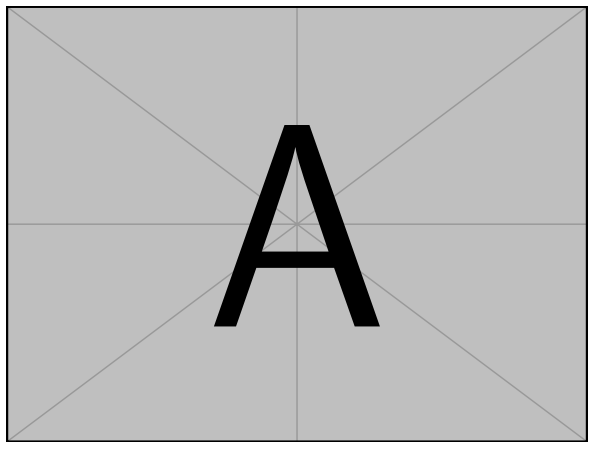
\includegraphics[width = 0.25\linewidth, angle = 135]{figures/A.png}
        \caption{Left-aligned}
    \end{subfigure}
    \\

    \begin{subfigure}{\linewidth}
        \centering
        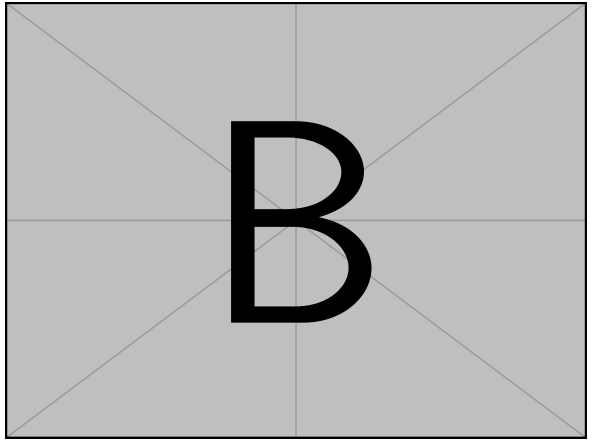
\includegraphics[width=0.4\linewidth]{figures/B.png}
        \caption{Center-aligned}
    \end{subfigure}
    \\
    
    \begin{subfigure}{\linewidth}
        \hfill
        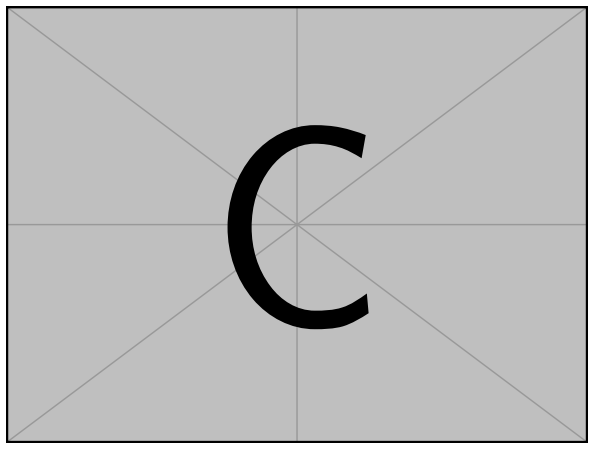
\includegraphics[width = 0.25\linewidth, angle = 45]{figures/C.png}
        \caption{Right-aligned}
    \end{subfigure}
    \caption{Three-row subfigure layout using for alignment}
    \label{fig:subfigs}
\end{figure}

Figure \ref{fig:subfigs} demonstrates left, center and right alignment using subfigures along with scaling and rotation.
\pagebreak

\section{Conclusion}
This document demonstrates \textbf{structured technical writing} using \LaTeX with \textit{diverse examples}, including tables, figures and equations. Students should pay attention to \underline{consistent layout}, \textbf{accurate alignment} and \textit{correct formatting} to achieve {\Large top marks}.

These extra lines give further clarification and guidance for understanding the material. They are plain text presented without any additional formatting.
\end{document}